% LaTeX Template for short student reports.
% Citations should be in bibtex format and go in references.bib
\documentclass[a4paper, 11pt]{article}
\usepackage[top=3cm, bottom=3cm, left=2cm, right=2cm]{geometry} 
\geometry{a4paper} 
\usepackage[utf8]{inputenc}
\usepackage[vietnamese]{babel}
\usepackage{textcomp}
\usepackage{graphicx} 
\usepackage{amsmath,amssymb}
\usepackage{algorithm,algcompatible}
\usepackage{caption}
\usepackage{bm}
\usepackage{tikz}
\usepackage{tabularx}
\usepackage{enumitem}
\setlist[itemize]{leftmargin=*}
\usepackage[pdftex,bookmarks,colorlinks,breaklinks]{hyperref}  
%\hypersetup{linkcolor=black,citecolor=black,filecolor=black,urlcolor=black} % black links, for printed output
\usepackage{graphicx}
\usepackage{memhfixc} 
\usepackage{pdfsync}
\usepackage{fancyhdr}
\usepackage{array}
\usepackage{listings}
\usepackage{xcolor}
\usepackage{float}

\pagestyle{fancy}
\setlength{\parindent}{0pt}
\graphicspath{ {images/} }
\setlength{\headheight}{16.50983pt}
\let\emptyset\varnothing

\definecolor{codegreen}{rgb}{0,0.6,0}
\definecolor{codegray}{rgb}{0.5,0.5,0.5}
\definecolor{codepurple}{rgb}{0.58,0,0.82}
\definecolor{backcolour}{rgb}{0.95,0.95,0.92}

\lstdefinestyle{mystyle}{
    backgroundcolor=\color{backcolour},   
    commentstyle=\color{codegreen},
    keywordstyle=\color{magenta},
    numberstyle=\tiny\color{codegray},
    stringstyle=\color{codepurple},
    basicstyle=\ttfamily\footnotesize,
    breakatwhitespace=false,         
    breaklines=true,                 
    captionpos=b,                    
    keepspaces=true,                 
    numbers=left,                    
    numbersep=5pt,                  
    showspaces=false,                
    showstringspaces=false,
    showtabs=false,                  
    tabsize=2
}
\lstset{style=mystyle}

\newenvironment{vnalgorithm}[1][]
  {\begin{algorithm}[#1]
     \selectlanguage{vietnamese}%
     \floatname{algorithm}{Thuật toán}%
     \algnewcommand\INPUT{\item[\textbf{Đầu vào:}]}%
     \algnewcommand\OUTPUT{\item[\textbf{Đầu ra:}]}%
     \algnewcommand\BEGIN{\item[\textbf{begin}]}
     \algnewcommand\RETURN{\State\textbf{return}}%
     \algnewcommand\BREAK{\State\textbf{break}}%
     \algnewcommand\CONTINUE{\State\textbf{continue}}
     \algnewcommand\END{\item[\textbf{end}]}%
     % Set other language requirements
  }
  {\end{algorithm}}

\title{Bài tập tuần 3}
\author{Nguyễn Lê Ngọc Duy}
\date{}

\begin{document}
\maketitle
\tableofcontents

\pagebreak

\section{Giới thiệu}

Bài tập tuần này sử dụng các thuật toán duyệt đồ thị như Breadth-first search (BFS), Depth-first search (DFS) và Uniform Cost Search (UCS) để giải quyết bài toán tìm đường đi ngắn nhất từ ĐHKHTN (đỉnh $V_{1}$) đến Sân bay TSN (đỉnh $V_{18}$) trên đồ thị sau:

\begin{figure}[h]
    \centering
    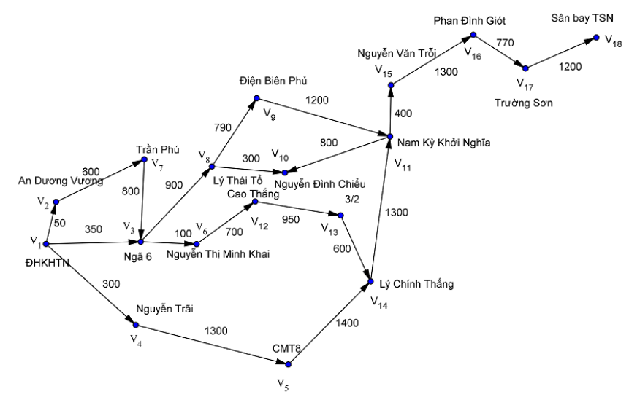
\includegraphics[]{problem.png}
    \caption{Đồ thị cho bài toán}
\end{figure}
\clearpage

\section{Giới thiệu các thuật toán}

\subsection{Thuật toán BFS}

Dưới đây là mô tả cho thuật toán BFS

\begin{vnalgorithm}
    \caption{Thuật toán Breadth First Search - BFS}
    \begin{algorithmic}[1]
        \INPUT{đồ thị $G$, node xuất phát $start$, node kết thúc $end$.}
        \OUTPUT{đường đi từ $start$ đến $end$}
        \BEGIN
            \STATE{Khởi tạo danh sách $L$ chứa trạng thái ban đầu.}
            \WHILE{true}
                \IF{$L$ rỗng}
                    \STATE{Thông báo không có đường đi.}
                    \BREAK
                \ENDIF
            \ENDWHILE
            \STATE{Loại trạng thái $u$ ở đầu danh sách $L$.}
            \IF{$u$ là trạng thái kết thúc}
                \RETURN{đường đi từ $start$ đến $u$.}
            \ENDIF
            \STATE{Lấy các trạng thái $v$ kề với $u$ và thêm vào cuối danh sách $L$.}
            \FOR{mỗi trạng thái $v$ kề với $u$}
                \STATE{$father(v) = u;$}
            \ENDFOR
        \END
    \end{algorithmic}
\end{vnalgorithm}

Áp dụng thuật toán BFS, ta giải quyết bài toán ở trên bằng bảng như sau:

\begin{center}
    \begin{tabular}{ |c|c|c| }
        \hline
        Lần lặp & Đỉnh & Hàng đợi\\
        \hline
        1 & $V_{1}$ (node bắt đầu) & $V_{2}, V_{3}, V_{4}$ \\
        \hline
        2 & $V_{2}$ & $V_{3}, V_{4}, V_{7}$ \\
        \hline
        3 & $V_{3}$ & $V_{4}, V_{7}, V_{6}, V_{8}$\\
        \hline
        4 & $V_{4}$ & $V_{7}, V_{6}, V_{8}, V_{5}$\\
        \hline
        5 & $V_{7}$ & $V_{6}, V_{8}, V_{5}$ \\
        \hline
        6 & $V_{6}$ & $V_{8}, V_{5}, V_{12}$  \\
        \hline
        7 & $V_{8}$ & $V_{5}, V_{12}, V_{9}, V_{10}$  \\
        \hline
        8 & $V_{5}$ & $V_{12}, V_{9}, V_{10}, V_{14}$ \\
        \hline
        9 & $V_{12}$ & $V_{9}, V_{10}, V_{14}, V_{13}$ \\
        \hline
        10 & $V_{9}$ & $V_{10}, V_{14}, V_{13}, V_{11}$  \\
        \hline
        11 & $V_{10}$ & $V_{14}, V_{13}, V_{11}$ \\
        \hline
        12 & $V_{14}$ & $V_{13}, V_{11}$ \\
        \hline
        13 & $V_{13}$ & $V_{11}$  \\
        \hline
        14 & $V_{11}$ & $V_{15}$ \\
        \hline
        15 & $V_{15}$ & $V_{16}$ \\
        \hline
        16 & $V_{16}$ & $V_{17}$ \\
        \hline
        17 & $V_{17}$ & $V_{18}$ \\
        \hline
        18 & $V_{18}$ (node kết thúc) & $\emptyset$ \\
        \hline
    \end{tabular}
\end{center}

Ta thu được đường đi theo thuật toán BFS là:
\begin{center}
    $V_{1} \rightarrow V_{4}  \rightarrow V_{5} \rightarrow V_{14} \rightarrow V_{11} \rightarrow V_{15} \rightarrow V_{16} \rightarrow V_{17} \rightarrow V_{18}$
\end{center}

\subsection{Thuật toán Depth First Search - DFS}
Dưới đây là mô tả cho thuật toán DFS
\begin{vnalgorithm}
    \caption{Thuật toán Depth First Search - DFS}
    \begin{algorithmic}[1]
        \INPUT{đồ thị $G$, node xuất phát $start$, node kết thúc $end$.}
        \OUTPUT{đường đi từ $start$ đến $end$}
        \BEGIN
            \STATE{Khởi tạo danh sách $L$ chứa trạng thái ban đầu.}
            \WHILE{true}
                \IF{$L$ rỗng}
                    \STATE{Thông báo không có đường đi.}
                    \BREAK
                \ENDIF
            \ENDWHILE
            \STATE{Loại trạng thái $u$ ở đầu danh sách $L$.}
            \IF{$u$ là trạng thái kết thúc}
                \RETURN{đường đi từ $start$ đến $u$.}
            \ENDIF
            \STATE{Lấy các trạng thái $v$ kề với $u$ và thêm vào đầu danh sách $L$.}
            \FOR{mỗi trạng thái $v$ kề với $u$}
                \STATE{$father(v) = u$}
            \ENDFOR
        \END
    \end{algorithmic}
\end{vnalgorithm}

Áp dụng thuật toán DFS, ta giải quyết bài toán trên bằng bảng như sau:
\begin{center}
    \begin{tabular}{ |c|c|c| }
        \hline
        Lần lặp & Đỉnh & Ngăn xếp\\
        \hline
        1 & $V_{1}$ (node xuất phát) & $V_{2}, V_{3}, V_{4}$ \\
        \hline
        2 & $V_{2}$ & $V_{7}, V_{3}, V_{4}$ \\
        \hline
        3 & $V_{7}$ & $V_{3}, V_{4}$ \\
        \hline
        4 & $V_{3}$ & $V_{6}, V_{8}, V_{4}$ \\
        \hline
        5 & $V_{6}$ & $V_{12}, V_{8}, V_{4}$ \\
        \hline
        6 & $V_{12}$ & $V_{13}, V_{8}, V_{4}$ \\
        \hline
        7 & $V_{13}$ & $V_{14}, V_{8}, V_{4}$ \\
        \hline
        8 & $V_{14}$ & $V_{11}, V_{8}, V_{4}$ \\
        \hline
        9 & $V_{11}$ & $V_{15}, V_{8}, V_{4}$\\
        \hline
        10 & $V_{15}$ & $V_{16}, V_{8}, V_{4}$\\
        \hline
        11 & $V_{16}$ & $V_{17}, V_{8}, V_{4}$\\
        \hline
        12 & $V_{17}$ & $V_{18}, V_{8}, V_{4}$ \\
        \hline
        13 & $V_{18}$ (node kết thúc) & $V_{8}, V_{4}$ \\
        \hline
    \end{tabular}
\end{center}

Ta thu được đường đi theo thuật toán DFS là:
\begin{center}
    $V_{1} \rightarrow V_{3} \rightarrow V_{6} \rightarrow V_{12} \rightarrow V_{13} \rightarrow V_{14} \rightarrow V_{11} \rightarrow V_{15} \rightarrow V_{16} \rightarrow V_{17} \rightarrow V_{18}$
\end{center}

\subsection{Thuật toán UCS}
Dưới đây là mô tả cho thuật toán UCS
\begin{vnalgorithm}
    \caption{Thuật toán Uniform Cost Search - UCS}
    \begin{algorithmic}[1]
        \INPUT{đồ thị $G$, node xuất phát $start$, node kết thúc $end$.}
        \OUTPUT{đường đi từ $start$ đến $end$ và chi phí của đường đi}
        \BEGIN
            \STATE{Tạo hàng đợi ưu tiên rỗng $NganChua$.}
            \STATE{Thêm nút $start$ vào $NganChua$.}
            \LOOP
                \IF{$NganChua$ rỗng}
                    \RETURN{không tồn tại đường đi.}
                \ELSE
                    \STATE{$Nut$ = TimChiPhiNhoNhat($NganChua$) }
                    \IF{KiemTraCauHoiDich($BaiToan$) trên TrangThai($Nut$) đúng}
                        \RETURN LoiGiai($Nut$)
                    \ENDIF
                \ENDIF
            \ENDLOOP
            \STATE {$LoiGiai$ = Mo($Nut$, $BaiToan$)}
            \STATE {$NganChua$ = ThemTatCa($LoiGiai$, $NganChua$)}
        \END
    \end{algorithmic}
\end{vnalgorithm}

Áp dụng thuật toán UCS, ta giải quyết bài toán trên bằng bảng như sau:
\begin{center}
    \begin{tabular}{ |c|c|c|c| }
        \hline
        Lần lặp & Đỉnh & Hàng đợi ưu tiên (theo thứ tự tổng chi phí) & Tổng chi phí thấp nhất \\
        \hline
        1 & $V_{1}$ (đỉnh bắt đầu) & $(V_{2}; 50)^*, (V_{4}; 300), (V_{3}; 350)$ & 50 \\
        \hline
        2 & $V_{2}$ & $(V_{4}; 300)^*, (V_{3}; 350), (V_{7}; 650)$ & 300 \\
        \hline
        3 & $V_{4}$ & $(V_{3}; 350)^*, (V_{7}; 650), (V_{5}; 1600)$ & 350 \\
        \hline
        4 & $V_{3}$ & $(V_{6}; 450)^*, (V_{7}; 650), (V_{5}; 1600), (V_{8}; 1250)$  & 450 \\
        \hline
        5 & $V_{6}$ & $(V_{7}; 650)^*, (V_{12}; 1150), (V_{8}; 1250), (V_{5}; 1600)$ & 650 \\
        \hline
        6 & $V_{7}$ & $(V_{12}; 1150)^*, (V_{8}; 1250), (V_{5}; 1600)$ & 1150 \\
        \hline
        7 & $V_{12}$ & $(V_{8}; 1250)^*, (V_{5}; 1600), (V_{13}; 2100)$ & 1250 \\
        \hline
        8 & $V_{8}$ & $(V_{10}; 1550)^*, (V_{5}; 1600), (V_{9}; 2040), (V_{13}; 2100)$ & 1550\\
        \hline
        9 & $V_{10}$ & $(V_{5}; 1600)^*, (V_{9}; 2040), (V_{13}; 2100)$ & 1600 \\
        \hline
        10 & $V_{5}$ & $(V_{9}; 2040)^*, (V_{13}; 2100), (V_{14}; 3000)$ & 2040 \\
        \hline
        11 & $V_{9}$ & $(V_{13}; 2100)^*, (V_{14}; 3000), (V_{11}; 3240)$ & 2100 \\
        \hline
        12 & $V_{13}$ & $(V_{14}; 2700)^*, (V_{11}; 3240)$ & 2700 \\
        \hline
        13 & $V_{14}$ & $(V_{11}; 3240)^*$ & 3240 \\
        \hline
        14 & $V_{11}$ & $(V_{15}, 3640)^*$ & 3640 \\
        \hline
        15 & $V_{15}$ & $(V_{16}, 4940)^*$ & 4940 \\
        \hline
        16 & $V_{16}$ & $(V_{17}, 5710)^*$ & 5710 \\
        \hline
        17 & $V_{17}$& $(V_{18}, 6910)^*$ & 6910 \\
        \hline
        18 & $V_{18}$ (đỉnh kết thúc) & $\emptyset$ & 6910 \\
        \hline
    \end{tabular}
\end{center}
Ta thu được đường đi theo thuật toán UCS (với tổng chi phí nhỏ nhất là 6910) như sau:
\begin{center}
    $V_{1} \xrightarrow{350} V_{3} \xrightarrow{900} V_{8} \xrightarrow{790} V_{9} \xrightarrow{1200} V_{11} \xrightarrow{400} V_{15} \xrightarrow{1300} V_{16} \xrightarrow{770} V_{17} \xrightarrow{1200} V_{18}$
\end{center}
\clearpage

\section{Cài đặt các thuật toán}

\subsection{Ngôn ngữ lập trình}
Ngôn ngữ lập trình dùng để cài đặt là ngôn ngữ lập trình Python, phiên bản 3.9.13.

\subsection{Cài đặt bằng phương pháp lập trình hàm}

\subsubsection{Dữ liệu đầu vào}
Dữ liệu đầu vào được lưu trữ trong 2 file \lstinline{input.txt} và \lstinline{input_ucs.txt} với định dạng như sau:

\begin{figure}[h]
    \centering
    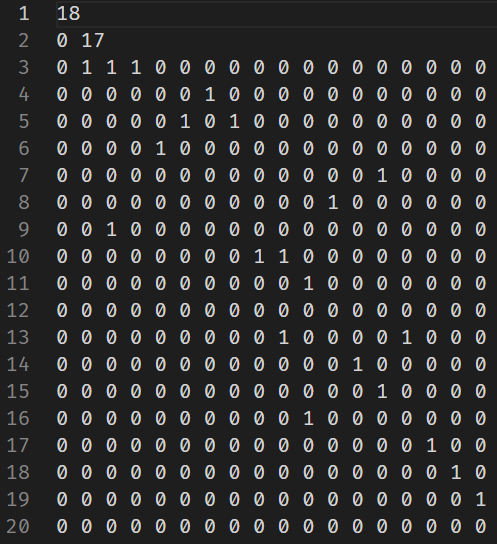
\includegraphics[]{input.png}
    \caption{Định dạng file đầu vào (không bao gồm trọng số) dùng cho thuật toán BFS và DFS}
\end{figure}

\begin{figure}[h]
    \centering
    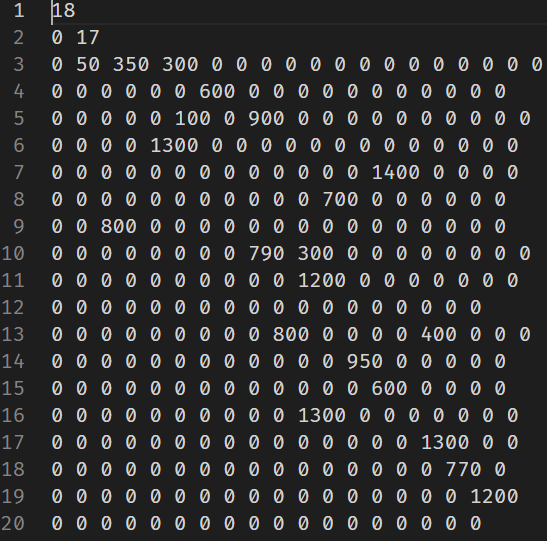
\includegraphics[]{input_ucs.png}
    \caption{Định dạng file đầu vào (bao gồm trọng số) dùng cho thuật toán UCS}
\end{figure}
\clearpage

\subsubsection{Các hàm phụ trợ}
Các hàm phụ trợ được định nghĩa trong file \lstinline{utilities.py} như sau:

\begin{lstlisting}[language=Python]
# Doc du lieu tu file text
def read_txt(file):
    size = int(file.readline())
    start, goal = [int(num) for num in file.readline().split(' ')]
    matrix = [[int(num) for num in file.readline().split(' ')] for num in range(size)]
    return size, start, goal, matrix

# Chuyen ma tran thanh danh sach ke
def convert_graph(a):
    adjList = defaultdict(list)
    for i in range(len(a)):
        for j in range(len(a[i])):
            if a[i][j] == 1:
                adjList[i].append(j)
    return adjList

def convert_graph_weight(a):
    adjList = defaultdict(list)
    for i in range(len(a)):
        for j in range(len(a[i])):
            if a[i][j] != 0:
                adjList[i].append((j, a[i][j]))
    return adjList
\end{lstlisting}

\subsubsection{Cài đặt thuật toán BFS}

Thuật toán BFS ban đầu được cài đặt bằng hàm \lstinline{bfs} trong file \lstinline{bfs.py} sau:

\begin{lstlisting}[language=Python]
def bfs(graph, start, end):
    visited = []
    frontier = Queue()

    # Them node start vao frontier va visited
    frontier.put(start)
    visited.append(start)

    # Node start khong co node cha
    parent = dict()
    parent[start] = None

    path_found = False

    while True:
        if frontier.empty():
            raise Exception("No path found")
        current_node = frontier.get()
        visited.append(current_node)

        # Kiem tra current_node co la node end khong
        if current_node == end:
            path_found = True
            break

        for node in graph[current_node]:
            if node not in visited:
                frontier.put(node)
                parent[node] = current_node
                visited.append(node)

    # Xay dung duong di
    path = []
    if path_found:
        path.append(end)
        while parent[end] is not None:
            path.append(parent[end])
            end = parent[end]
        path.reverse()
        
    return path
\end{lstlisting}

\begin{figure}[h]
    \centering
    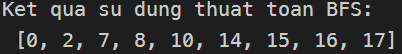
\includegraphics[]{bfs_func.png}
    \caption{Kết quả của hàm bfs}
\end{figure}

\subsubsection{Cài đặt thuật toán DFS}
Thuật toán DFS ban đầu được cài đặt bằng hàm \lstinline{dfs} trong file \lstinline{dfs.py} sau:

\begin{lstlisting}[language=Python]
def dfs(graph, start, end):
    visited = []
    frontier = []

    # Them node start vao frontier va visited
    frontier.append(start)
    visited.append(start)

    # start khong co node cha
    parent = dict()
    parent[start] = None

    path_found = False
    while True:
        if frontier == []:
            raise Exception("No path found")
        current_node = frontier.pop()
        visited.append(current_node)

        # Kiem tra current_node co la node end khong
        if current_node == end:
            path_found = True
            break

        for node in graph[current_node]:
            if node not in visited:
                frontier.append(node)
                parent[node] = current_node
                visited.append(node)
    
    # Xay dung duong di
    path = []
    if path_found:
        path.append(end)
        while parent[end] is not None:
            path.append(parent[end])
            end = parent[end]
        path.reverse()
    
    return path
\end{lstlisting}

\begin{figure}[h]
    \centering
    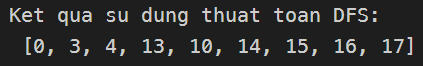
\includegraphics[]{dfs_func.png}
    \caption{Kết quả của hàm dfs}
\end{figure}

\subsubsection{Cài đặt thuật toán UCS}
Thuật toán UCS ban đầu được cài đặt bằng hàm \lstinline{ucs} trong file \lstinline{ucs.py} sau:
\begin{lstlisting}[language=Python]
def ucs(graph, start, end):
    visited = []
    frontier = PriorityQueue()

    # Them node start vao frontier va visited
    frontier.put((0, start))
    visited.append(start)

    # Node start khong co node cha
    parent = dict()
    parent[start] = None

    path_found = False
    while True:
        if frontier.empty():
            raise Exception("No path found")
        current_weight, current_node = frontier.get()
        visited.append(current_node)

        # Kiem tra current_node co la node end khong
        if current_node == end:
            path_found = True
            break

        for node_i in graph[current_node]:
            node, weight = node_i
            if node not in visited:
                frontier.put((current_weight + weight, node))
                parent[node] = current_node
                visited.append(node)

    # Xay dung duong di
    path = []
    if path_found:
        path.append(end)
        while parent[end] is not None:
            path.append(parent[end])
            end = parent[end]
        path.reverse()
    
    return current_weight, path
\end{lstlisting}

\begin{figure}[h]
    \centering
    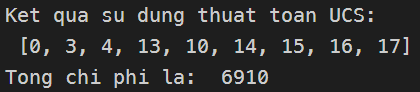
\includegraphics[]{ucs_func.png}
    \caption{Kết quả của hàm ucs}
\end{figure}

\subsection{Xây dựng lớp Graph riêng}
Để thuận tiện hơn, thay vì cài đặt riêng các hàm rời rạc như trên, ta có thể xây dựng một lớp \lstinline{Graph} và cài đặt tất cả các hàm vào trong lớp này để thuận tiện cho việc khởi tạp đối tượng và chạy các thuật toán. Lớp \lstinline{Graph} được cài đặt trong file \lstinline{graph.py} sau:

\begin{lstlisting}[language=Python]
from queue import Queue, PriorityQueue
from collections import defaultdict


class Graph:
    def __init__(self):
        self.adjancy_matrix = None
        self.adjancy_list = None
        self.start_node = None
        self.end_node = None
        self.has_weight = False
        self.size = 0

    def read_file_text(self, file_name="input.txt"):
        file = open(file_name, "r")
        self.size = int(file.readline())
        self.start_node, self.end_node = [int(num) for num in file.readline().split(' ')]
        self.adjancy_matrix = [[int(num) for num in file.readline().split(' ')] for num in range(self.size)]
        return self.size, self.start_node, self.end_node, self.adjancy_matrix

    def write_file_text(self, file_name="output.txt"):
        file = open(file_name, "w")
        pass

    def convert_to_list(self, weight=None):
        self.adjancy_list = defaultdict(list)
        for i in range(len(self.adjancy_matrix)):
            for j in range(len(self.adjancy_matrix[i])):
                if self.adjancy_matrix[i][j] == 1 and weight is None:
                    self.adjancy_list[i].append(j)
                if self.adjancy_matrix[i][j] != 0 and weight is not None:
                    self.adjancy_list[i].append((j, self.adjancy_matrix[i][j]))
                    self.has_weight = True
        return self.adjancy_list

    def dfs(self, start_node, end_node):
        visited = []
        frontier = []

        frontier.append(start_node)
        visited.append(start_node)

        parent = dict()
        parent[start_node] = None

        path_found = False
        while True:
            if frontier == []:
                raise Exception("No path found")
            current_node = frontier.pop()
            visited.append(current_node)

            if current_node == end_node:
                path_found = True
                break

            for node in self.adjancy_list[current_node]:
                if node not in visited:
                    frontier.append(node)
                    parent[node] = current_node
                    visited.append(node)

        path = []
        if path_found:
            path.append(end_node)
            while parent[end_node] is not None:
                path.append(parent[end_node])
                end_node = parent[end_node]
            path.reverse()

        return path

    def bfs(self, start_node, end_node):
        visited = []
        frontier = Queue()

        frontier.put(start_node)
        visited.append(start_node)

        parent = dict()
        parent[start_node] = None

        path_found = False

        while True:
            if frontier.empty():
                raise Exception("No path found")
            current_node = frontier.get()
            visited.append(current_node)

            if current_node == end_node:
                path_found = True
                break

            for node in self.adjancy_list[current_node]:
                if node not in visited:
                    frontier.put(node)
                    parent[node] = current_node
                    visited.append(node)
        
        path = []
        if path_found:
            path.append(end_node)
            while parent[end_node] is not None:
                path.append(parent[end_node])
                end_node = parent[end_node]
            path.reverse()

        return path

    def ucs(self, start_node, end_node):
        visited = []
        frontier = PriorityQueue()

        frontier.put((0, start_node))
        visited.append(start_node)

        parent = dict()
        parent[start_node] = None

        path_found = False
        
        while True:
            if frontier.empty():
                raise Exception("No path found")
            current_weight, current_node = frontier.get()
            visited.append(current_node)

            if current_node == end_node:
                path_found = True
                break

            for node_i in self.adjancy_list[current_node]:
                node, weight = node_i
                if node not in visited:
                    frontier.put((current_weight + weight, node))
                    parent[node] = current_node
                    visited.append(node)

        path = []
        if path_found:
            path.append(end_node)
            while parent[end_node] is not None:
                path.append(parent[end_node])
                end_node = parent[end_node]
            path.reverse()

        return path, current_weight
\end{lstlisting}

\begin{figure}[h]
    \centering
    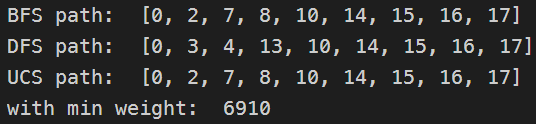
\includegraphics[]{graph.png}
    \caption{Kết quả các thuật toán sau khi cài đặt class Graph}
\end{figure}

\section{Nhận xét}
- Kết quả đường đi của các thuật toán tìm kiếm đường đi trên đồ thị vô hướng không có trọng số và có trọng số khi chạy tay đều không giống với kết quả sau khi code.

- Trọng số thấp nhất của thuật toán UCS sau khi chạy trên máy giống với kết quả khi chạy tay.

- Thuật toán BFS ưu tiên duyệt node theo chiều rộng (theo thứ tự từ trái sang phải) nên đường đi của nó sẽ ngắn hơn so với DFS.

- Thuật toán UCS ưu tiên duyệt node theo chiều sâu nhưng ưu tiên duyệt node có trọng số thấp nhất nên đường đi của nó sẽ có tổng chi phí thấp hơn nhiều so với BFS.

% \bibliography{references}  % need to put bibtex references in references.bib 
\end{document}